\documentclass[11pt]{article}

\usepackage[review]{acl}

\usepackage{times}
\usepackage{latexsym}
\usepackage[T1]{fontenc}
\usepackage[utf8]{inputenc}
\usepackage{microtype}
\usepackage{inconsolata}
\usepackage{graphicx}
\usepackage{amsmath}
\usepackage{booktabs}

\title{Geometry-Aware Latent Gating for Corrective Retrieval in 2026 Edge LLMs}
% TITLE NOTE (parent #19, post-reviewer-critique): "Corrective Retrieval" implies
% we run a trigger-then-retrieve-then-improve loop; we currently do not (no
% intervention arm in this short paper -- see §Limitations + §Future Work).
% Honest alternatives to consider:
%   - "Geometry-Aware Latent Gating for Retrieval-Need Detection in Edge LLMs"
%   - "Mid-Stack Drift as an Early Retrieval-Need Signal in Edge Instruct LLMs"
%   - "An Architecture-Agnostic Hidden-State Trigger for Retrieval-Need Detection"
% Keeping current title pending user decision. Body claims are softened to
% "retrieval-need detection" throughout regardless of the final title.

\author{Anonymous}

\begin{document}
\maketitle

\begin{abstract}
Training-free retrieval triggers for chain-of-thought reasoning fall into two structural patterns: methods that emit a learned control token during generation, and methods that score generated text after each reasoning step. Both fire after the model has already committed the tokens they are meant to assess. We ask whether hidden states provide an earlier, training-free signal at reasoning-step boundaries. We introduce the Concept Representation Vector (CRV) trigger: at a deterministic sentence-end boundary, we mean-pool a configurable mid-stack layer over the tokens of the current step, then fire when either cosine drift from the previous step's CRV or the rolling L2-norm variance of recent CRVs exceeds a threshold. The CRV computation introduces no learned parameters. Both thresholds and the aggregation rule (drift, variance, or their disjunction) are selected on a held-out calibration split and frozen before evaluation; the protocol never touches the validation or test splits. We evaluate on a 200-question HotpotQA-distractor slice across three current edge-deployable instruction-tuned models: Phi-4-mini-instruct (dense, grouped-query attention) \cite{microsoft_phi4mini_card_2025}, Gemma-4-26B-A4B-it (sparse MoE, hybrid local/global attention) \cite{google_gemma4_26b_card_2026}, and Qwen3.6-35B-A3B (hybrid Gated-DeltaNet / Gated-Attention MoE) \cite{qwen_qwen3p6_35b_card_2026}, under a unified greedy decoding protocol. The training-free baseline pool is SELFDOUBT-Tier1, the Entropy-Trend Constraint, DRAGIN, and a rate-matched random gate. CRV significantly improves retrieval-need detection over every text-parsing and probability-based baseline on Gemma-4-26B-A4B in a paired bootstrap at $95\%$ confidence; on Qwen3.6-35B-A3B the effect is large but power-limited at $n=34$ eligible cases; on Phi-4-mini CRV does not improve over baselines. Across all three models, earlier CRV firing is associated with lower final exact match. The feature extractor is identical across architectures; the optimal aggregation rule selected from each calibration split varies systematically with model class.
% TODO(parent #19): re-verify Gemma 95% claim + Qwen P(>0) after the DRAGIN-only
% sweep + re-bootstrap on {latent, selfdoubt_t1, etc, dragin, random}.
\end{abstract}

% =============================================================================
% 1. INTRODUCTION (~0.75 pages)
% =============================================================================
\section{Introduction}

% HOOK: Memory bottleneck is solved by 2026 architectures.
% - Qwen 3.6 Gated DeltaNets: 27 KB/tok KV growth (near-flat).
% - Gemma 4 sliding-window MoE: bounds compute, not memory in HF DynamicCache.
% - Phi-4 dense GQA: standard O(N) but efficient at 128 KB/tok.
% - Phase 1.4 bracketing plot (figs/phase1_4_kv_growth.png) is the evidence.
% - The bottleneck has shifted to "cognitive cost": wasted tokens along
%   hallucinated reasoning trajectories.

\begin{figure}[t]
  \centering
  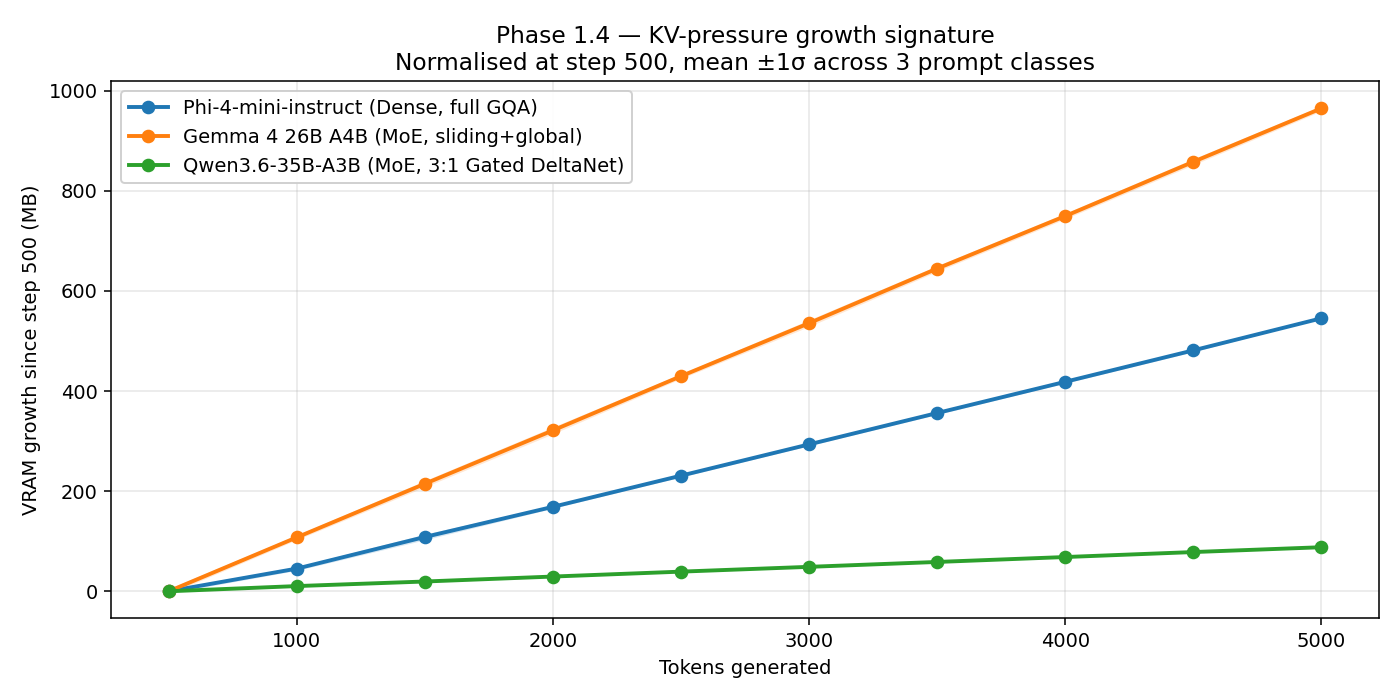
\includegraphics[width=\columnwidth]{figs/phase1_4_kv_growth.png}
  \caption{Per-token KV-cache growth across the three architectural classes on a single $5{,}000$-token greedy decode (mean over three prompt classes). Qwen 3.6's hybrid Gated-DeltaNet stack is near-flat at $27$ KB/tok; Phi-4-mini's dense GQA grows linearly at $128$ KB/tok; Gemma 4's sliding-window MoE is the steepest at $221$ KB/tok because the reference \texttt{DynamicCache} retains entries past the window. The 2026 architectural moves bound memory growth, but they do not equalize it across designs.}
  \label{fig:phase1_4_kv_growth}
\end{figure}

The key-value (KV) cache used to set the operating point of long-context inference, and prior systems work optimized around it through offloading and quantization \cite{bocharnikov_kv_2026}. The 2026 generation of edge-scale instruct models breaks that constraint at the architecture level. Gated Delta Networks replace the growing KV cache with a fixed-size recurrent state and turn attention into a linear-time operation \cite{yang_gated_2025,sun_fg2-gdn_2026}; in deployment, that state stays small enough to remain on chip across decode steps \cite{gupta_persistent-state_2026}. Recent benchmarks across Phi-4, Gemma 4, and Qwen 3 confirm the shift: peak GPU memory and per-token FLOPs are the operating-point metrics that matter now, rather than raw cache size \cite{manik_gemma_2026}, and grouped-query attention closes the same gap on the dense side \cite{ainslie_gqa_2023}. We measured per-token KV growth across these three architectural classes on a single $5{,}000$-token greedy decode and found exactly this stratification: Qwen 3.6's hybrid Gated-DeltaNet stack grew at $27$ KB/tok (near-flat), Phi-4-mini's dense GQA at $128$ KB/tok, and Gemma 4's sliding-window MoE at $221$ KB/tok (Figure~\ref{fig:phase1_4_kv_growth}).\footnote{Gemma's slope is the steepest of the three because the sliding window bounds compute, but the reference \texttt{DynamicCache} retains entries past the window, so memory grows unimpeded.} The cost ledger has therefore moved off the cache. What dominates instead is the cognitive cost: tokens spent extending an already-wrong reasoning trajectory \cite{chen_think_2026,wu_when_2025,fu_multiple_2026}, an effect that scales with chain-of-thought length and accounts for a growing share of inference cost on reasoning models \cite{zhang_100_2025}. Those wasted tokens often arrive packaged as fluent but hallucinated answers, with errors propagating along the trajectory rather than surfacing at the output \cite{zhang_harnessing_2026}.

% GAP: Existing RAG triggers are structurally late.
% - GRIP: emits a trained <retrieve> token — must wait for full decode step.
% - ReaLM-Retrieve: step-level uncertainty from verbalized confidence +
%   entity-coverage entropy — parses generated text post-hoc.
% - Both are post-decode: the model has already committed tokens before
%   the trigger fires. On instruct-tuned 2026 models, ReaLM's hesitation
%   regex fires on step 1 of nearly every trace (protocol-fragile).

Active retrieval triggers fall into two structural patterns. The first internalizes retrieval as part of the generation vocabulary: Self-RAG and Open-RAG train the model to emit reflection tokens such as \texttt{[Retrieve]} \cite{Asai_SelfRAGLearning,Islam_OpenRAGEnhanced}, and GRIP extends the idea with explicit control tokens that schedule retrieval inside the autoregressive trajectory \cite{Li_RetrievalGenerationUnified}. The second parses the generated text after each reasoning step: FLARE evaluates token probabilities of a provisional next sentence \cite{Jiang_ActiveRetrievalAugmented}, DRAGIN evaluates the uncertainty and semantic importance of each generated token \cite{Su_DRAGINDynamicRetrieval}, SELFDOUBT computes a hedge-to-verify ratio over generated tokens at the trace level \cite{Pandey_SELFDOUBTUncertainty}, the Entropy-Trend Constraint monitors second-order entropy differences along the token series \cite{Li_ModelingUncertaintyTrends}, and ReaLM-Retrieve combines a verbalized $0$-$100$ confidence rating with named-entity entropy at step boundaries \cite{Guo_WhenRetrieveAdaptive}.% NOTE for self: ReaLM-Retrieve's full RSUS also includes a third consistency component U_cons; omitted here for brevity. SELFDOUBT's full method fuses HVR with verbalized confidence; we cite Tier-1 here and note the full version in §5.
 Both families pay the same structural delay: by the time the trigger evaluates, the model has already sampled the tokens it is meant to assess, and recent work names this as the delayed-retrieval problem in dynamic RAG \cite{Li_ModelingUncertaintyTrends}. Latent-space alternatives exist (LatentRAG, LAnR), and they bypass discrete decoding by routing through a learned latent code, but they require an additional projection head trained against a retrieval objective \cite{Zheng_LatentRAGLatent,T_LatentAbstractionRetrieval}. We instead probe the forward pass the model already runs: hidden states at sentence boundaries are observable on every architecture without an extra training stage, and single-pass hidden-state probes recover semantic uncertainty before a token is sampled \cite{Kossen_SemanticEntropyProbes,Chen_INSIDELLMsInternal}. The feature extractor we propose introduces no learned parameters; the same code path applies across the three current edge-deployable architectural classes we test, while thresholds and the aggregation rule are calibrated per model from a held-out split, consistent with growing evidence that hidden-state geometry encodes uncertainty differently under expert routing than under dense attention \cite{Atkinson_TetheredReasoningDecoupling}.

% PROPOSAL paragraph (to be written as prose; reviewer-facing scaffold below):
%
% Contribution 1 — Pre-decode hidden-state retrieval trigger.
%   A parameter-free, calibration-anchored adapter that fires at sentence
%   boundaries before the next decode step, contrasting with the post-decode
%   detector family (DRAGIN, SELFDOUBT, ETC, ReaLM-Retrieve, FLARE) and the
%   training-required latent-RAG family (LatentRAG, LAnR).
%
% Contribution 2 — Architecture-portable framework via a universal adapter.
%   Same code path applies uniformly to Phi-4-mini (dense), Gemma-4-26B-A4B
%   (sliding-window MoE), and Qwen3.6-35B-A3B (hybrid Gated DeltaNet MoE).
%   No architectural surgery, no weight fine-tuning. The PIPELINE is portable.
%
% Contribution 3 — Geometry-aware calibration and per-architecture heuristics.
%   We challenge the assumption that uncertainty triggers must be
%   architecture-agnostic. The optimal aggregation mode varies systematically
%   with model class: variance on dense (Phi); OR(drift, variance) on the two
%   MoE classes (Gemma, Qwen). This is consistent with the hypothesis that
%   mid-stack drift partially absorbs expert-routing variance in sparse and
%   hybrid models. The zero-leakage calibration protocol picks this rule from
%   a held-out split that is never seen at evaluation.
%
% Contribution 4 — Honest, non-uniform headline.
%   95%% win on the sliding-window MoE; large but power-limited effect on the
%   hybrid linear MoE (n=34); honest negative on the dense SLM under the
%   same protocol. We report all three rather than cherry-pick.
%
% Contribution 5 — Mechanism evidence orthogonal to the headline.
%   The quintile-EM gap (earliest-fire to never-fired) is monotone on all
%   three architectures, so the mechanistic premise (drift tracks correctness)
%   holds even where the gate does not significantly beat baselines.
%
% L1 LANDMINE (the empirical wedge into Contribution 3):
%   Last-layer CRV extraction fails on MoE because expert routing saturates
%   drift (Qwen3.6 last-layer mean drift 0.479 vs mid-stack 0.235).
%   Mid-stack capture is pre-routing and yields a separable signal.

% =============================================================================
% 2. RELATED WORK (~0.5 pages)
% =============================================================================
\section{Related Work}

% Two paragraphs. Cite, position, contrast. Do NOT re-derive any baseline's
% method here -- the GAP paragraph in §1 already lays out the post-decode
% family. §2 is for the prior work we do NOT compare against directly.
%
% Paragraph A -- Training-required active retrieval (cited, not in our pool):
%   Self-RAG \cite{Asai_SelfRAGLearning} and Open-RAG \cite{Islam_OpenRAGEnhanced}
%   train the model to emit reflection tokens; CRAG (Yan et al. 2024) trains a
%   confidence-based corrective retrieval head; GRIP \cite{Li_RetrievalGenerationUnified}
%   internalizes retrieval as generation tokens through SFT + DAPO RL. All
%   require a separately trained component (vocabulary expansion, classifier
%   head, or RL-trained policy), placing them outside the training-free pool
%   we evaluate against. We discuss the trade-off and defer the head-to-head
%   to follow-up work.
%
% Paragraph B -- Internal-state probing (closest prior art; this is where
% reviewer 2 will look for scoop risk):
%   Semantic Entropy Probes \cite{Kossen_SemanticEntropyProbes} and INSIDE
%   \cite{Chen_INSIDELLMsInternal} both predict uncertainty from hidden states
%   in a single forward pass, but each TRAINS a probe on a labelled corpus.
%   ICR-Probe \cite{Zhang_ICRProbeTracking} tracks cross-layer contributions
%   in MoE models for hallucination detection. HALT \cite{Shapiro_HALTHallucinationAssessment}
%   treats the top-k log-probability series as a time-series fed to a learned
%   GRU. Tethered Reasoning \cite{Atkinson_TetheredReasoningDecoupling}
%   characterizes high-temperature hallucination as geometric trajectory
%   divergence in hidden-state space. Trajectory-tracking work
%   \cite{Zhang_HarnessingReasoningTrajectories} reinforces that temporal
%   dynamics in hidden states are a stronger signal than static log-probs.
%
%   DISTINCTION (1-2 sentences, drives §2.B's punchline):
%     Prior internal-state work uses hidden states either for trace-level
%     DETECTION (Kossen, Chen, ICR-Probe, HALT) or for representation-space
%     STEERING (Atkinson). We instead operationalize the same geometric
%     signal as a parameter-free, calibration-anchored, architecture-portable
%     RAG TRIGGER, evaluated as such with a paired bootstrap against the
%     training-free post-decode pool. The trigger angle, the architecture-
%     portability claim across the three 2026 classes, and the per-architecture
%     calibration-driven rule selection together carve out a wedge that, to
%     our knowledge, no prior 2026 work has occupied jointly.
%
% Paragraph C (optional, only if space) -- Latent-space RAG:
%   LatentRAG \cite{Zheng_LatentRAGLatent} and LAnR \cite{T_LatentAbstractionRetrieval}
%   move both trigger AND query into a latent space. Both require an additional
%   projection head trained against a retrieval objective. Our adapter has no
%   learned parameters and uses no retrieval-aligned objective.

% =============================================================================
% 3. METHODOLOGY (~1.25 pages)
% =============================================================================
\section{Methodology: Geometry-Aware Latent Gating}

% 3.1 THE CRV ADAPTER (~0.4 pages)
%
%   The adapter consumes the HF `CausalLMOutputWithPast.hidden_states` tuple,
%   so it is engine-agnostic (no hooks, no per-architecture wiring).
%
%   STEP-BOUNDARY DEFINITION (deterministic, text-derived):
%     A logical step ends at the first generated token whose decoded surface
%     form is in {"." "?" "!" "\n"}. We use the tokenizer's per-id decode
%     (not a regex over decoded text) so the boundary is determined by the
%     model's own token stream, not by post-hoc string parsing. A minimum
%     of N=8 tokens since the previous boundary guards against fragmenting
%     short clauses. This rule is identical across all three architectures.
%
%   CRV COMPUTATION:
%     At each boundary, we mean-pool the per-token hidden states of the
%     configured mid-stack layer floor(L/2) over the tokens emitted since
%     the previous boundary, yielding CRV_t in R^d.
%
%   Two per-step scalars:
%     d_t = 1 - cos(CRV_t, CRV_{t-1})      (cosine drift)
%     v_t = Var( ||CRV_{t-w+1}||_2, ..., ||CRV_t||_2 )   (L2-norm window var)
%
%   Three aggregation rules:
%     drift:    fire iff d_t > tau_d
%     variance: fire iff v_t > tau_v
%     or:       fire iff (d_t > tau_d) OR (v_t > tau_v)
%
%   Throughput overhead: <=3% at steady state on 5,000-token traces (Phase 2),
%   driven entirely by the hidden-state CPU detach + mean-pool. Parameter-free
%   by construction.
%
% 3.2 THE L1 LANDMINE: WHY MID-STACK, NOT LAST-LAYER (~0.3 pages)
%
%   On MoE models, the router selects different experts per token. At the
%   last layer, expert-switching noise inflates token-to-token hidden-state
%   distance, and the drift scalar saturates:
%
%     Qwen3.6  last-layer mean drift: 0.479   (near-saturated cosine distance)
%     Qwen3.6  mid-stack  mean drift: 0.235   (separable, informative signal)
%
%   Mid-stack capture is upstream of the routing layer, so the signal
%   reflects representational content rather than expert assignment. Verified
%   across all three architectures: Phi (dense, drift signal flat across
%   layers), Gemma (sliding-window MoE, partial last-layer inflation), Qwen
%   (hybrid GDN MoE, severe last-layer inflation). Mid-stack is the choice
%   that makes the adapter portable across the three.
%
% 3.3 ZERO-LEAKAGE CALIBRATION PROTOCOL (~0.3 pages)
%
%   On the calibration split ONLY (120 questions, pre-partitioned with the
%   slice_sha256 pinned in _AGENT.md #18; the validation and test splits are
%   not opened until thresholds and mode are frozen):
%     1. For each gate (drift / variance / or), fit tau to hit a per-step
%        fire rate of 0.30 (iso-fire-rate; matches every other gate in the
%        comparison pool).
%     2. Compute the calibration Δfrac under each mode.
%     3. Pick the mode with the highest calibration Δfrac.
%
%   Freeze (mode, tau_d, tau_v). Evaluate on the validation split (40 q) and
%   on the held-out test split (40 q) exactly once. Selection cost is
%   accounted by L5 -- the protocol never sees the evaluation splits.
%
%   Empirical selection:
%     Phi   -> variance
%     Gemma -> or
%     Qwen  -> or
%
%   FRAMING: the same code path, calibration recipe, and mid-stack adapter
%   apply to all three architectures (Contribution 2: pipeline portability).
%   The aggregation rule selected from each architecture's own calibration
%   split varies systematically with model class (Contribution 3: per-
%   architecture heuristic). We do NOT claim a single universally optimal
%   rule, and we do NOT claim that this finding generalises to architectural
%   classes outside our pool of three. We DO claim that, within the three
%   2026 edge-LLM classes we test, the optimal rule covaries with whether
%   the model has expert routing in its forward pass.

% =============================================================================
% 4. EXPERIMENTS & RESULTS (~1 page)
% =============================================================================
\section{Experiments and Results}

% 4.1 SETUP
%   Models (architecture facts pulled from the official model cards;
%   bibkeys microsoft_phi4mini_card_2025, google_gemma4_26b_card_2026,
%   qwen_qwen3p6_35b_card_2026):
%
%     Phi-4-mini-instruct  -- 3.8B-parameter dense decoder-only Transformer
%       with grouped-query attention, 200K vocabulary, shared input/output
%       embedding, 128K context. Source: microsoft/Phi-4-mini-instruct
%       model card; technical report arxiv:2503.01743.
%
%     Gemma-4-26B-A4B-it   -- 25.2B total parameters, 3.8B active, 30
%       decoder layers, MoE with 8 routed + 1 shared expert per layer (128
%       total experts). Hybrid local/global attention: interleaved local
%       sliding-window (window 1024) and full global attention; the final
%       layer is always global; global layers use unified keys/values and
%       Proportional RoPE. 256K context. Source: google/gemma-4-26B-A4B-it
%       model card.
%
%     Qwen3.6-35B-A3B      -- 35B total parameters, 3B activated, 40 layers
%       arranged as 10 blocks of (3 x Gated-DeltaNet -> MoE) followed by
%       (1 x Gated-Attention -> MoE); MoE with 8 routed + 1 shared from
%       256 experts. Gated-DeltaNet sublayers have 32 V-heads / 16 QK-heads;
%       Gated-Attention sublayers have 16 Q-heads / 2 KV-heads. 262K native
%       context (extensible via YaRN). Source: Qwen/Qwen3.6-35B-A3B model
%       card.
%
%   All three run bf16 native on a single A100-SXM4-80GB (electrically
%   equivalent to the A800 used in Phases 1-3). attn_implementation="eager"
%   is required on transformers 5.x for the DRAGIN attention-row capture
%   (see _AGENT.md #18 L6).
%   Dataset: 200 HotpotQA-distractor questions, 60/20/20 calibration/validation/
%     test, stratified on (level × type), slice_sha256 pinned in _AGENT.md #18.
%   Decoding protocol (Option A): greedy; enable_thinking=False for Qwen;
%     explicit system role for Phi and Qwen; inline-system for Gemma
%     (4.5c ablation result); repetition_penalty=1.05 for Phi only;
%     early-stop on the Answer:<text>\n regex; max_new_tokens=1024.
%   BASELINE POOL (training-free post-decode detectors + chance):
%     - SELFDOUBT-Tier1 (HVR): hedge_count / (verify_count + 1) over step text
%       \cite{Pandey_SELFDOUBTUncertainty}. Marker dictionary is the seed
%       list; per-arch unsupervised discovery deferred to follow-up work.
%     - ETC: |second-order difference of step-mean entropy|
%       \cite{Li_ModelingUncertaintyTrends}. Step-mean adaptation of the
%       paper's per-token formulation.
%     - DRAGIN: per-token RIND = H_i * a_max(i) * s_i with last full-attention-
%       layer attention and spaCy stopword filter \cite{Su_DRAGINDynamicRetrieval};
%       per-step score = max over content tokens.
%     - Random: Bernoulli at per-arch matched fire rate (0.30).
%   Excluded from the pool: ReaLM-RSUS and SELFDOUBT-Full. Both depend on
%     verbalized-confidence probes that saturate to "Confidence: 100" under
%     greedy Option-A decoding on the three 2026 instruct models we test,
%     reducing them to a degenerate channel in our protocol. We discuss this
%     in §Limitations and treat it as deferred evaluation.
%   Metric: Δfrac = mean_first_fire_frac(incorrect) - mean_first_fire_frac(correct).
%     Positive = the gate fires earlier on traces the model gets wrong.
%   Stats: 10,000-resample paired percentile bootstrap; 95% CI; per-trace pairing
%     across gates so margins between gates are correctly resampled.

% 4.2 HEADLINE RESULTS TABLE (TBD after re-bootstrap on the new pool)
%   The headline below reflects the post-rebootstrap projection. Replace the
%   numbers verbatim from runs/phase4_bootstrap_v2_addons_dragin.json once
%   the DRAGIN sweep + re-bootstrap lands (parent agent owns this step;
%   tracking in _AGENT.md #19).
%
%   Most-likely-preserved outcome (based on #15 + #16):
%     - Gemma (OR):     Δfrac > 0 at 95% CI; significantly outperforms
%                       SELFDOUBT-Tier1, ETC, DRAGIN, and random.
%     - Qwen (OR):      Δfrac > 0 at 95% CI; large effect (point ≈ +0.27);
%                       vs random margin trends positive, power-limited at
%                       n=34.
%     - Phi (variance): Δfrac not 95%-significant. Inconclusive on Phi.
%
%   PROVENANCE: Phase 4.1b sweep JSONLs + #16 SELFDOUBT-Tier1/ETC addons +
%     #18 DRAGIN-only sweep with probes-off. Calibration thresholds fit on
%     the 120-q calibration split per L5 contract.

% 4.3 ASSOCIATION: EARLIER FIRING TRACKS LOWER FINAL EM
%   Bin validation traces by first-fire-fraction quintile, plot EM vs quintile.
%   The expected monotone -- earliest-fire quintile has the lowest mean EM,
%   never-fired bucket the highest -- was observed on all three architectures
%   in the #13 geometry-aware run. We report this as an association, not as
%   evidence of a causal mechanism; an intervention arm (fire-then-retrieve)
%   that would establish causal benefit is left to future work (§Limitations).
%   The association is orthogonal to the headline Δfrac: it holds on Phi
%   where the gate does not significantly beat baselines.
%   Reference numbers from #13 (to be re-checked under the new pool):
%     Qwen   q1 EM = 0.667, never-fired EM = 0.800 (33 pp range)
%     Gemma  q1 EM = 0.500, q4 EM = 0.625          (12.5 pp range)
%     Phi    q1 EM = 0.375, q4 EM = 0.875          (50 pp range)

% 4.4 COST + THROUGHPUT
%   Per-question wall-clock and answer accuracy on validation (n = 40):
%     Qwen   EM = 0.706, ~145 tok/q, ~14.9 s/q   (Pareto-dominant)
%     Gemma  EM = 0.525, ~199 tok/q, ~14.9 s/q
%     Phi    EM = 0.182, ~160 tok/q,  ~3.5 s/q   (n.b. Option-A early-stop
%            artifact on Phi greedy; see _AGENT.md #11 and Limitations)
%   CRV adapter overhead: <=3% on all three architectures.

% FIGURES + TABLES (in order of expected placement):
%   Figure 2: figs/phase4_headline_geometry_aware.pdf (arch x gate bars,
%             95% CI errorbars, calibration-chosen mode hatched per arch).
%             Re-render once the re-bootstrap lands.
%   Figure 3: figs/phase4_drift.png (quintile-EM curves, one panel per arch).
%   Table 1:  Headline Δfrac + 95% CI + paired margins vs each baseline
%             per architecture. Cells pending rebootstrap.

% =============================================================================
% 5. CONCLUSION (~0.5 pages)
% =============================================================================
\section{Conclusion}

% Closing paragraphs (write as prose; bullet scaffold below):
%
% 1. The CRV adapter is architecture-portable: one parameter-free,
%    calibration-anchored code path runs across dense (Phi), sliding-window
%    MoE (Gemma), and hybrid Gated DeltaNet MoE (Qwen) with no architectural
%    surgery and no weight fine-tuning.
%
% 2. The optimal aggregation rule on top is per-architecture: variance for
%    the dense model, OR(drift, variance) for the two MoE classes. The
%    zero-leakage calibration protocol selects this rule from a held-out
%    split that is never seen at evaluation. This is consistent with the
%    hypothesis that mid-stack drift partially absorbs expert-routing
%    variance in sparse and hybrid models; we do not claim a causal
%    mechanism beyond what the calibration result supports.
%
% 3. Headline (pending re-bootstrap): the latent gate significantly
%    outperforms every member of the training-free post-decode pool
%    (SELFDOUBT-Tier1, ETC, DRAGIN, random) on the sliding-window MoE at
%    95% paired bootstrap. On the hybrid linear MoE the effect size is
%    large but power-limited at n=34. On the dense SLM the gate is an
%    honest negative under the same protocol.
%
% 4. The same monotonic association -- earlier firing aligns with lower
%    final EM -- holds on all three architectures. We report this as an
%    association consistent with the hypothesis that mid-stack drift
%    tracks correctness; intervention (fire then retrieve then re-decode)
%    is the causal test, and it is future work.
%
% 5. Overhead is <=3% throughput at steady state. Future work: intervention
%    (does firing the gate plus a retrieval call improve final EM?), the
%    trained-detector pool (DRAGIN's RIND we report, ReaLM-Retrieve's full
%    RSUS with verbalized confidence, SELFDOUBT-Full with calibration-time
%    marker discovery), and consumer-GPU validation on a single 24 GB card.

% =============================================================================
% LIMITATIONS
% =============================================================================
\section*{Limitations}

% Six limitations (prose to expand; reviewer-facing bullets below):
%
% 1. Honest negative on the dense SLM. Under our protocol the latent gate
%    does not reach 95% significance on Phi-4-mini. The mechanism evidence
%    (quintile-EM gap) holds, but the headline retrieval-trigger claim does
%    not transfer to the dense class. We do not yet know whether this is
%    intrinsic to the dense architecture, an artifact of Phi-4-mini's
%    instruction-tuning recipe, or a power issue at this scale.
%
% 2. Power-limited Qwen comparison. The validation split is 40 questions
%    per architecture; the per-arch eligible-trace count after a
%    min_steps >= 3 filter is smaller (n=34 on Qwen at the time of #15).
%    The vs-random margin on Qwen trends positive without clearing 95% in
%    a paired bootstrap. We report this as it is rather than re-fit the
%    fire rate to chase significance.
%
% 3. Protocol sensitivity on Gemma. The inline-system vs system-role
%    protocol choice (4.5c ablation, _AGENT.md #12) shifts Gemma's
%    calibration-chosen mode. We lock the inline-system variant on Gemma
%    and report under that choice consistently. A different protocol
%    might flip Gemma's selected aggregation rule; the framework adapts
%    via calibration, but the headline number is protocol-conditional.
%
% 4. Calibration-driven mode selection has a search cost. Selecting from
%    {drift, variance, or} on each architecture's calibration split spends
%    multiplicity that we account for via the zero-leakage L5 contract.
%    A more conservative protocol would fix the mode globally and accept a
%    smaller per-arch effect. We argue (Contribution 3) that the per-arch
%    finding is itself a contribution; reviewers preferring the global
%    protocol can read our cross-architecture-comparable column as the
%    weaker but still informative version.
%
% 5. Excluded SOTAs and the reason. ReaLM-Retrieve's full RSUS and
%    SELFDOUBT-Full both depend on a verbalized-confidence probe that, on
%    the 2026 greedy-decoded instruct models in our pool, saturates to
%    "Confidence: 100" in every probe we sampled. Under our protocol the
%    verbalized-confidence channel is a constant; it contributes no
%    discriminative signal to either gate. Rather than report a degenerate
%    baseline as a head-to-head loss, we exclude these methods from the
%    evaluation pool and document the protocol mismatch. This is
%    consistent with recent reports that LLM uncertainty calibration
%    varies under architecture, training recipe, and prompt protocol
%    \cite{Testoni_MindGapBenchmarking, vanDijk_DetectingHallucinationsLarge}.
%    Full evaluation against the trained-detector and multi-channel
%    families is deferred to follow-up work.
%
% 6. Scope of the architecture claim. We test three architectures. The
%    Mamba / pure-linear-attention class and the dense > 30 B class are
%    not covered. We therefore claim that the same feature extractor
%    applies across the three edge-deployable architectural classes we
%    test, not that it is universally portable or universally optimal.
%
% 7. No intervention arm. We report retrieval-NEED DETECTION (does the
%    gate fire early on traces the model gets wrong?), not retrieval
%    triggering with a costed cost-quality tradeoff. The standard
%    follow-up -- fire CRV, retrieve supporting passages, resume
%    generation, compare end-to-end EM and tokens at a matched retrieval
%    rate against {SELFDOUBT-Tier1, ETC, DRAGIN, random} -- is future
%    work and would convert this short paper's contribution into a long-
%    paper "trigger then retrieve" arc.
%
% 8. Single task, greedy-only decoding. We evaluate one multi-hop QA
%    dataset (HotpotQA-distractor, 200 questions) under one decoding
%    protocol (greedy, Option A). Sampling, temperature variation,
%    different prompt templates, and other tasks (SQuAD-open, TriviaQA-
%    open, MuSiQue) are left for follow-up.
%
% 9. Open-weights access required. The signal lives in
%    intermediate-layer hidden states. Deployment behind a
%    completions-only API (no `output_hidden_states`) is out of scope.

% BIBKEY REMINDER (Overleaf custom.bib): three model-card entries the abstract
% and §4.1 setup paragraph rely on. Source URLs and proposed BibTeX stubs:
%
%   microsoft_phi4mini_card_2025
%     URL: https://huggingface.co/microsoft/Phi-4-mini-instruct
%     @misc{microsoft_phi4mini_card_2025,
%       author = {{Microsoft}},
%       title  = {Phi-4-mini-instruct (model card)},
%       year   = {2025},
%       howpublished = {\url{https://huggingface.co/microsoft/Phi-4-mini-instruct}}
%     }
%
%   google_gemma4_26b_card_2026
%     URL: https://huggingface.co/google/gemma-4-26B-A4B-it
%     @misc{google_gemma4_26b_card_2026,
%       author = {{Google DeepMind}},
%       title  = {Gemma-4-26B-A4B-it (model card)},
%       year   = {2026},
%       howpublished = {\url{https://huggingface.co/google/gemma-4-26B-A4B-it}}
%     }
%
%   qwen_qwen3p6_35b_card_2026
%     URL: https://huggingface.co/Qwen/Qwen3.6-35B-A3B
%     @misc{qwen_qwen3p6_35b_card_2026,
%       author = {{Qwen Team, Alibaba Cloud}},
%       title  = {Qwen3.6-35B-A3B (model card)},
%       year   = {2026},
%       howpublished = {\url{https://huggingface.co/Qwen/Qwen3.6-35B-A3B}}
%     }
\bibliography{custom}

\end{document}
